\section*{Тестирование программы}

\subsection*{Создание матрицы}

На рис. \ref{matrix_creation1} представленно создание матрицы 5х10 с помощью 1 пункта меню.

\begin{figure}[hpt!]
	\centering
	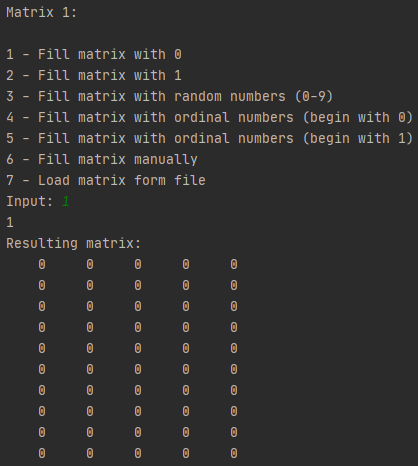
\includegraphics[width=0.6\linewidth]{photo/matrix_creation1}
	\caption{Создание матрицы с помощью 1 пункта меню}
	\label{matrix_creation1}
\end{figure}

\newpage

На рис. \ref{matrix_creation2} представленно создание матрицы 5х10 с помощью 2 пункта меню.

\begin{figure}[hpt!]
	\centering
	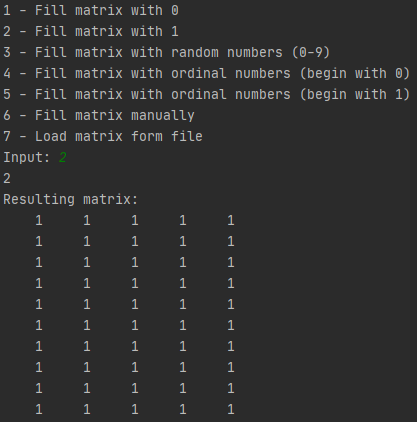
\includegraphics[width=0.6\linewidth]{photo/matrix_creation2}
	\caption{Создание матрицы с помощью 2 пункта меню}
	\label{matrix_creation2}
\end{figure}

\newpage

На рис. \ref{matrix_creation3} представленно создание матрицы 4х7 с помощью 3 пункта меню.

\begin{figure}[hpt!]
	\centering
	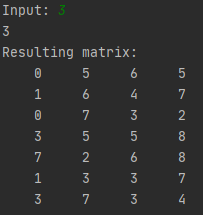
\includegraphics[width=0.6\linewidth]{photo/matrix_creation3}
	\caption{Создание матрицы с помощью 3 пункта меню}
	\label{matrix_creation3}
\end{figure}

\newpage

На рис. \ref{matrix_creation4} представленно создание матрицы 4х7 с помощью 4 пункта меню.

\begin{figure}[hpt!]
	\centering
	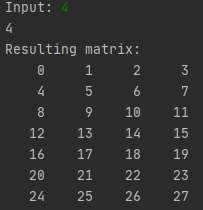
\includegraphics[width=0.6\linewidth]{photo/matrix_creation4}
	\caption{Создание матрицы с помощью 4 пункта меню}
	\label{matrix_creation4}
\end{figure}

\newpage

На рис. \ref{matrix_creation5} представленно создание матрицы 9х11 с помощью 5 пункта меню.

\begin{figure}[hpt!]
	\centering
	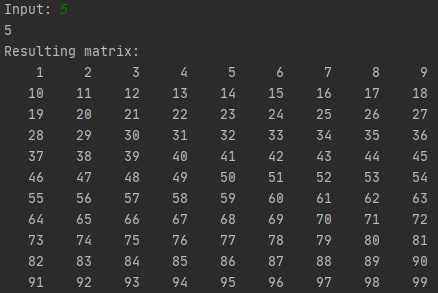
\includegraphics[width=0.6\linewidth]{photo/matrix_creation5}
	\caption{Создание матрицы с помощью 5 пункта меню}
	\label{matrix_creation5}
\end{figure}

\newpage

На рис. \ref{matrix_creation6.1}, \ref{matrix_creation6.2} 
представленно создание матрицы 4х4 с помощью 6 пункта меню.

\begin{figure}[hpt!]
	\centering
	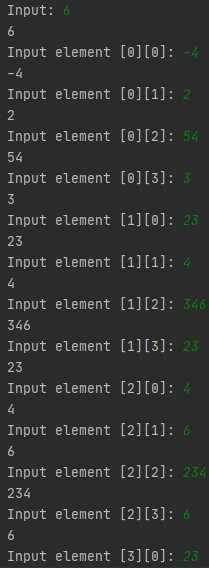
\includegraphics[width=0.5\linewidth]{photo/matrix_creation6.1}
	\caption{Создание матрицы с помощью 6 пункта меню (1)}
	\label{matrix_creation6.1}
\end{figure}

\begin{figure}[hpt!]
	\centering
	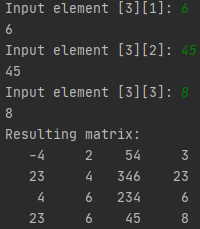
\includegraphics[width=0.6\linewidth]{photo/matrix_creation6.2}
	\caption{Создание матрицы с помощью 6 пункта меню (2)}
	\label{matrix_creation6.2}
\end{figure}

\newpage

На рис. \ref{matrix_creation7.fail} представленно создание матрицы с помощью 7 пункта меню. 
Вводилось заведомо неверное расположение файла, после чего было получено ожидаемое сообщение об ошибке.

\begin{figure}[hpt!]
	\centering
	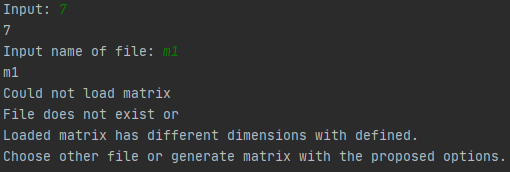
\includegraphics[width=0.6\linewidth]{photo/matrix_creation7.fail}
	\caption{Создание матрицы с помощью 7 пункта меню (неверный файл)}
	\label{matrix_creation7.fail}
\end{figure}

\newpage

На рис. \ref{matrix_creation7.success} представленно создание матрицы с помощью 7 пункта меню.
Вводилось заведомо верное расположение файла, после чего была получена ожидаемая матрица.

\begin{figure}[hpt!]
	\centering
	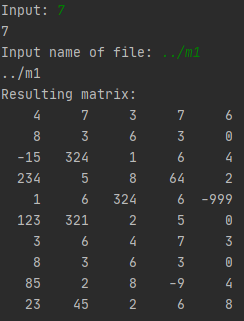
\includegraphics[width=0.6\linewidth]{photo/matrix_creation7.success}
	\caption{Создание матрицы с помощью 7 пункта меню (верный файл)}
	\label{matrix_creation7.success}
\end{figure}

\newpage

\subsection*{Суммирование матриц}

На рис. \ref{sum1} показаны результаты теста №1.

\begin{figure}[hpt!]
	\centering
	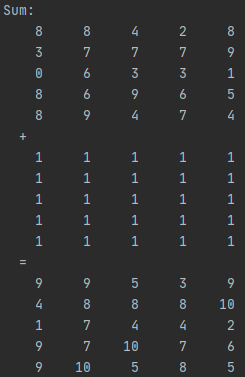
\includegraphics[width=0.6\linewidth]{photo/sum1(5x5)}
	\caption{Тест №1}
	\label{sum1}
\end{figure}

На рис. \ref{sum2} показаны результаты теста №2.

\begin{figure}[hpt!]
	\centering
	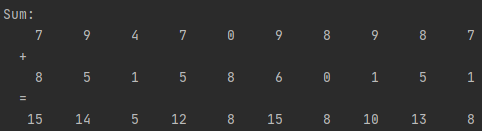
\includegraphics[width=0.6\linewidth]{photo/sum2(10x1)}
	\caption{Тест №1}
	\label{sum2}
\end{figure}

\newpage

На рис. \ref{sum3} показаны результаты теста №3.

\begin{figure}[hpt!]
	\centering
	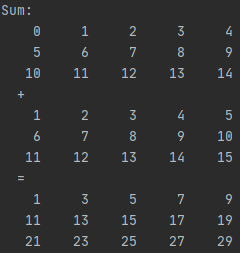
\includegraphics[width=0.6\linewidth]{photo/sum3(5x3)}
	\caption{Тест №1}
	\label{sum3}
\end{figure}